\subsubsection{Projetos com manipuladores industriais fixos}\label{proj_manip}
Há diversos manipuladores robóticos industriais com as especificações
necessárias para a realização da tarefa de metalização por HVOF. As empresas
Fanuc, Motoman, ABB e KUKA fabricam manipuladores com dimensões compatíveis com o
acesso pela escotilha inferior e velocidade, precisão, e espaço de trabalho que
cumprem os requisitos para a execução do processo em todo um lado da pá, em uma
base fixa. Porém, há incompatibilidade atrás da pá e a necessidade de escolher a
posição correta do manipulador em relação à pá, a fim de maximizar a sua área de trabalho, no ambiente da
turbina, o que pode restringir os seus movimentos.
Como as pás podem ser giradas até um ângulo de $14.5^o$, são discutidas as ideias de posicionamento
do manipulador entre as pás, a fim de executar a operação em ambos os lados da
pá (um lado de cada pá), e o posicionamento fixo à frente e depois atrás à pá.

\paragraph{Posicionamento entre pás}

A figura~\ref{fig::andaime} mostra o espaço entre as pás da turbina, dentro do
aro câmara. Um robô manipulador de médio porte pode ser fixado em uma base
magnética, na posição que se encontra a escada da figura~\ref{fig::andaime}.
Essa posição é vantajosa por possibilitar a execução da tarefa em duas pás
(frente de uma e verso da outra), sem desmontar ou fazer grandes alterações no
posicionamento da base do robô, diminuindo as intervenções e tempo de tarefa.
 
\begin{figure}[h!]
\centering
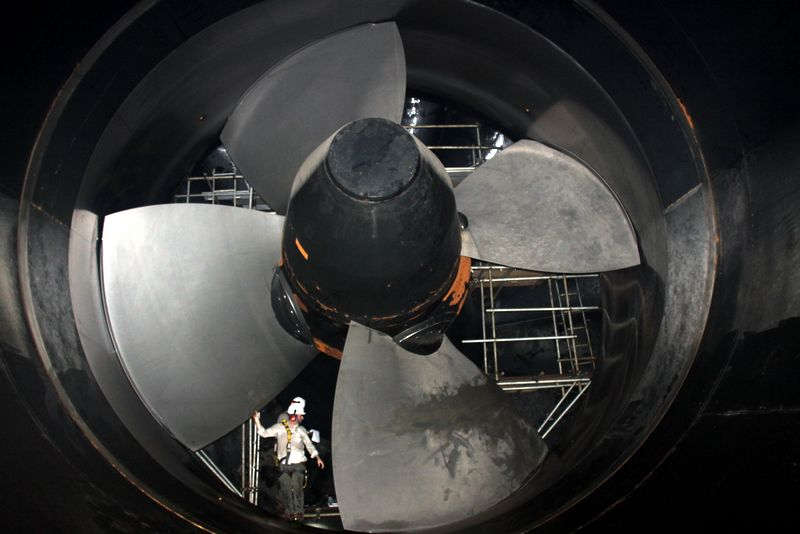
\includegraphics[width=0.7\textwidth]{figs/andaime.jpg}
\caption{Espaço entre as pás da turbina.}
\label{fig::andaime}
\end{figure}

O estudo puramente geométrico demonstra que o alcance do manipulador robótico
para o processamento de ambos os lados das pás, considerando uma base fixa entre
as pás, deverá ser em torno de 5 metros. O manipulador industrial IRB5500,
desenvolvido pela ABB para pintura, possui 3 metros de alcance, porém 180 kg, o que já dificulta ou até impossibilita a
logística de movimentação e posicionamento in-situ. Não foi encontrado um robô
industrial com o alcance necessário e que tivesse as dimensões máximas da
escotilha inferior. 

A solução conceitual de posicionar um manipulador industrial entre as pás deve
avaliar, portanto, todas as configurações necessárias da base (orientações e
posições) para garantir que todo o espaço de trabalho do manipulador mais base
cubra os lados de ambas as pás. O número de configurações e o projeto
mecânico da base são necessários para a viabilização da solução,
uma vez que será possível avaliar as intervenções e complexidades. Bases
autônomas diminuem o número de intervenções e aumentam a precisção do sistema,
porém aumentam a complexidade, o custo devido ao número de sensores e atuadores,
e o peso do sistema, prejudicando a logística.

\paragraph{Posicionamento à frente e atrás da pá}

Posicionar de maneira fixa um manipulador com base magnética à frente e atrás da
pá para a metalização é uma solução natural, já que é semelhante à utilizada pela
empresa Rijeza atualmente. Um estudo puramente geométrico, utilizando as
dimensões da pá, mostra que o manipulador deve possuir alcance de 1.7 m e ser
posicionado a uma altura de 1.1 m em relação ao solo. Estudos de espaço de
trabalho, manipulabilidade e colisões devem ser realizados para confirmar o
estudo geométrico.

O posicionamento do sistema à frente ou atrás da pá exige intervenções para
rotação da turbina e para o deslocamento do sistema. Em relação a um
sistema com base autônoma entre as pás, o processo parece mais custoso em
intervenções manuais e mais demorado, porém bem mais simples em termos de
robótica.

\paragraph{Conclusão da solução com manipuladores industriais}
A utilização de manipuladores industriais é a mais simples, em termos de
sistemas robóticos, dentre todas as soluções para o acesso pela escotilha
inferior.
Não há projeto mecânico do manipulador, já que este será adquirido em um dos fabricantes citados. As dificuldades mecânicas do projeto serão em relação à logística de posicionamento
e movimentação do robô dentro do aro câmara, e no desenvolvimento de uma base,
que pode ser autônoma. Além disso, o projeto fica responsável pelo controle do
manipulador, processamento de dados que envolvem o HVOF, planejamento de
trajetórias e interface de usuário.

Os desafios consistem na construção de uma base rígida e a locomoção dos
equipamentos pelo aro câmara. Este projeto conceitual será uma das frentes para
o estudo de viabilidade.
